%%%%%%%%%%%%%%%%%%%%%%%%%%%%%%%%%%%%%%%%%%%%%%%%%%%%%%%%%%%%%%%%%%%%%%%
% BAB 5
%%%%%%%%%%%%%%%%%%%%%%%%%%%%%%%%%%%%%%%%%%%%%%%%%%%%%%%%%%%%%%%%%%%%%%%

\mychapter{5}{BAB 5 HASIL DAN PEMBAHASAN}

\section{Analisis Kebutuhan Pengujian}

Hasil pada tahapan ini berupa daftar \emph{method} yang akan
diuji. Daftar tersebut ditentukan oleh pembimbing lapangan dengan
beberapa pertimbangan, antra lain terbatasnya waktu praktik kerja
lapangan. Daftar \emph{method} yang akan diuji terlihat pada Tabel
\ref{tab:method-yang-diuji}

\begin{longtable}[c]{|l|l|p{2.5cm}|p{7cm}|}
  \caption{Daftar \emph{method} yang akan diuji} \label{tab:method-yang-diuji} \\
  %% HEADER
  \hline
  \textbf{Kode} & \textbf{Modul} & \textbf{\emph{Method}} & \textbf{Deskripsi} \\
  \hline
  \endhead % <-- on every page
  NC1 & attach & attach & Sistem menjalankan perintah
                                       pada \emph{remote virtual machine}\\\hline
                                       %
  NC2 & create & do\_create & Sistem membuat \emph{virtual machine} \\\hline
                                  %
  NC3 & auth & do\_login & Sistem mengautentikasi pengguna \\\hline
  %
  NC4 & auth & do\_logout & Sistem menghapus data autentikasi \emph{user}\\\hline
  %
  NC5 & ls & get\_stack\_list & Sistem menampilkan daftar \emph{stack} \\\hline
                        %
  NC6 & ls & list\_network & Sistem menampilkan daftar \emph{networks} \\\hline
                           %
  NC7 & vm & do\_delete & Sistem menghapus \emph{virtual machine}\\\hline
                            %
  NC8 & orch & do\_delete & Sistem menghapus \emph{stack}\\\hline
                                      %
  NC9 & orch & do\_update & Sistem memperbarui \emph{virtual machine}\\\hline
                               %
  NC10 & cli & show\_help & Sistem menampilkan pesan bantuan \\\hline
  %
  NC11 & cli & show\_version & Sistem dapat menampilkan versi perangkat lunak \\\hline
  %
\end{longtable}


%%% Local Variables:
%%% mode: latex
%%% TeX-master: "pkl"
%%% End:


\section{Perancangan dan Implementasi Kasus Uji}

\subsection{Kasus Uji NC1}

\subsubsection{Pengujian Unit \emph{ssh\_out\_stream}}

Pengujian \emph{unit} dilakukan pada \emph{method ssh\_out\_stream}
secara terisolasi dan sebagai \emph{stand-alone program}. Maka
dilakukan \emph{mocking} pada \emph{method exec\_command} dan
\emph{exit\_status\_ready}.

\begin{code}
\begin{ignasicblock}[title=ssh\_out\_stream,minted language=text]
procedure ssh_out_stream()
    exec_command(commands)                 (1)
    # infinite while
    WHILE True:                            (2)
        IF exit_status_ready():            (3)
            break                          (4)
        ENDIF                              (5)
        length = channel                   (6)
        IF length > 0:                     (7)
            print length                   (8)
        ENDIF                              (9)
    ENDWHILE                               (10)
end
\end{ignasicblock}
\captionof{listing}{\emph{Pseudocode} \emph{ssh\_out\_stream}}
\label{pc:ssh_out_stream}
\end{code}

\par\null\par
\noindent
\emph{Flow graph} yang dihasilkan dari \emph{pseudocode}
ssh\_out\_stream terlihat pada Gambar \ref{cfg:ssh_out_stream}.
\emph{Flow graph} tersebut memiliki nilai \emph{cyclomatic complexity} V(G) = 3 \emph{regions} = 3.

\begin{figure}[H]
  \centering
  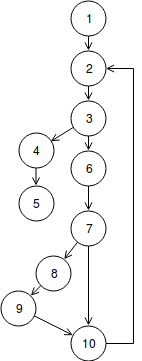
\includegraphics[width=.2\linewidth]{img/test-case/ssh_out_stream}
  \caption{\emph{Flow graph} dari \emph{pseudocode} \emph{ssh\_out\_stream}}
  \label{cfg:ssh_out_stream}
\end{figure}

\noindent
\emph{Independent Path}

\begin{enumerate}
\item Jalur 1 : 1 - 2 - 3 - 4 - 5
\item Jalur 2 : 1 - 2 - 3 - 6 - 7 - 10 - 2 - 3 - 4 - 5
\item Jalur 3 : 1 - 2 - 3 - 6 - 7 - 8 - 9 - 10 - 2 - 3 - 4 - 5
\end{enumerate}

\begin{longtable}{|P{.06\textwidth}|P{.30\textwidth}|P{.30\textwidth}|P{.10\textwidth}|P{.08\textwidth}|}
  \caption{Pengujian \emph{unit} \emph{ssh\_out\_stream}} \label{jalur:ssh_out_stream}\\
  \hline
  \textbf{Jalur} & \textbf{Prosedur Uji} &
                                                        \textbf{\emph{Expected Result}}
  & \textbf{\emph{Result}} & \textbf{Status} \\\hline
  %
  1 & Memberikan nilai \emph{true} pada \emph{variable}
      \emph{exit\_status\_ready()} & \emph{ssh\_out\_stream} berhenti berjalan & \emph{As expected} & Valid \\\hline
      %
  2 & Memberikan nilai lebih kecil dari 0 pada
      \emph{variable length} & \emph{ssh\_out\_stream} tidak menampilkan nilai \emph{variable} \emph{length}
  & \emph{As expected} & Valid \\\hline
  %
  3 & Memberikan nilai lebih besar dari 0 pada
      \emph{variable length} & \emph{ssh\_out\_stream} menampilkan nilai
                               \emph{variable} \emph{length} & \emph{As expected} & Valid \\\hline
  %
\end{longtable}

\subsubsection{Pengujian Integrasi \emph{attach}}

\begin{code}
\begin{ignasicblock}[title=attach,minted language=text]
procedure attach
TRY                                         (1)
    ssh__out_stream(commands)               (2)
EXCEPT
    exit                                    (3)
ENDTRY                                      (4)
end
\end{ignasicblock}
\captionof{listing}{\emph{Pseudocode} \emph{attach}}
\label{pc:attach-c}
\end{code}


\par\null\par
\noindent
\emph{Flow graph} yang dihasilkan dari \emph{pseudocode}
attach terlihat pada Gambar \ref{cfg:attach-c}. \emph{Flow graph} tersebut Memiliki
nilai \emph{cyclomatic complexity} V(G) = 2 \emph{regions} = 2.

\begin{figure}[H]
  \centering
  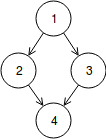
\includegraphics[width=.17\linewidth]{img/test-case/attach-c}
  \caption{\emph{Flow graph} dari \emph{pseudocode} \emph{attach}}
  \label{cfg:attach-c}
\end{figure}

\noindent
\emph{Independent Path}

\begin{enumerate}
\item Jalur 1 : 1 - 2 - 4
\item Jalur 2 : 1 - 3 - 4
\end{enumerate}

\begin{longtable}{|P{.06\textwidth}|P{.29\textwidth}|P{.29\textwidth}|P{.12\textwidth}|P{.08\textwidth}|}
  \caption{Pengujian \emph{integration} \emph{attach}} \label{jalur:attach-c} \\
  \hline
  \textbf{Jalur} & \textbf{Prosedur Uji} & \textbf{\emph{Expected Result}}
  & \textbf{\emph{Result}} & \textbf{Status} \\\hline
  %
  1 & Melakukan \emph{raise exception} & Sistem menjalankan perintah pada
                                         \emph{remote virtual machine} & \emph{As expected} & Valid \\\hline
                               %
  2 & Tidak Melakukan \emph{raise exception} & Sistem berhenti & \emph{As expected} & Valid \\\hline
      %
\end{longtable}

\subsubsection{\emph{Test Script} Untuk \emph{Automated Testing}}

\begin{code}
\begin{ignasicblock}[title=test\_attach\_command,minted language=Python]
@pytest.mark.run(order=3)
def test_attach_command(self):
    # neo.yml located inside tests dir
    os.chdir("tests")

    # wait until vm fully resized
    vm_status = ''
    while vm_status != 'ACTIVE':
        # get 'unittest-vm' id
        vm_data = vm_lib.get_list()
        for vm in vm_data:
            if vm.name == 'unittest-vm':
                vm_status = vm.status
                time.sleep(4)
                print('vm still updating ...')

    f = StringIO()
    with redirect_stdout(f):
        a = Attach({'<args>': ['-c', 'ls -a'],
                    '<command>': 'attach'}, '-c', 'ls -a')
        a.execute()
        out = f.getvalue()

    os.chdir(os.pardir)
    assert 'Success' in out
\end{ignasicblock}
\captionof{listing}{\emph{Test script} untuk \emph{attach}}
\label{ts:attach-c}
\end{code}

\subsection{Kasus Uji NC2}

\subsubsection{Pengujian Unit \emph{get\_heat\_client}}

\noindent
Pengujian \emph{unit} dilakukan pada \emph{method get\_heat\_client}
secara terisolasi dan sebagai \emph{stand-alone program}. Maka
dilakukan \emph{mocking} pada \emph{method load\_session} dan
\emph{heat\_client}.

\begin{code}
\begin{ignasicblock}[title=get\_heat\_client,minted language=text]
procedure get_heat_client()
    TRY                                 (1)
        IF not session:                 (2)
            session = load_session()
            heat = heat_client()
            return heat                 (3)
        ENDIF                           (4)
    EXCEPT
       show_error_log                   (5)
    ENDTRY                              (6)
end
\end{ignasicblock}
\captionof{listing}{\emph{Pseudocode} \emph{get\_heat\_client}}
\label{pc:get_heat_client}
\end{code}

\par\null\par
\noindent
\emph{Flow graph} yang dihasilkan dari \emph{pseudocode}
get\_heat\_client terlihat pada Gambar \ref{cfg:get_heat_client}.
\emph{Flow graph} tersebut memiliki nilai \emph{cyclomatic complexity} V(G) = 2 \emph{regions} = 2.

\begin{figure}[H]
  \centering
  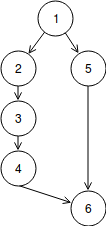
\includegraphics[width=.17\linewidth]{img/test-case/get_heat_client}
  \caption{\emph{Flow graph} dari \emph{pseudocode} \emph{get\_heat\_client}}
  \label{cfg:get_heat_client}
\end{figure}

\noindent
\emph{Independent Path}

\begin{enumerate}
\item Jalur 1 : 1 - 5 - 6
\item Jalur 1 : 1 - 2 - 3 - 4 - 6
\end{enumerate}

\begin{longtable}{|P{.06\textwidth}|P{.30\textwidth}|P{.30\textwidth}|P{.10\textwidth}|P{.08\textwidth}|}
  \caption{Pengujian \emph{unit} \emph{get\_heat\_client}} \label{jalur:get_heat_client} \\
  \hline
  \textbf{Jalur} & \textbf{Prosedur Uji} & \textbf{\emph{Expected Result}}
  & \textbf{\emph{Result}} & \textbf{Status} \\\hline
  1 & Memberikan nilai  \emph{raise exception} & Sistem menampilkan \emph{error log} dan
                               berhenti & \emph{As expected} & Valid \\\hline
                               %
  2 & Memberikan nilai \emph{false} pada \emph{variable session} & Sistem mengambil nilai
                                                                   \emph{session} dan mengembalikan nilai \emph{variable heat}
  & \emph{As expected} & Valid \\\hline
  %
\end{longtable}

\subsubsection{Pengujian Unit \emph{yaml\_parser}}

Pengujian \emph{unit} pada \emph{method yaml\_parser} dilakukan secara
terisolasi. Maka dilakukan \emph{mocking} pada \emph{method load} \\

\begin{code}
\begin{ignasicblock}[title=yaml\_parser,minted language=text]
procedure yaml_parser()
    TRY                             (1)
        data = load_file            (2)
        return data
    EXCEPT
        show_error_log              (3)
    ENDTRY
end
\end{ignasicblock}
\captionof{listing}{\emph{Pseudocode} \emph{yaml\_parser}}
\label{pc:yaml_parser}
\end{code}

\par\null\par
\noindent
\emph{Flow graph} yang dihasilkan dari \emph{pseudocode}
yaml\_parser terlihat pada Gambar \ref{cfg:yaml_parser}. \emph{Flow graph} tersebut memiliki
nilai \emph{cyclomatic complexity} V(G) = 2 \emph{regions}  = 2.

\begin{figure}[H]
  \centering
  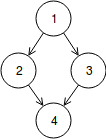
\includegraphics[width=.17\linewidth]{img/test-case/attach-c} %sama 4 biji
  \caption{\emph{Flow graph} dari \emph{pseudocode} \emph{yaml\_parser}}
  \label{cfg:yaml_parser}
\end{figure}

\noindent
\emph{Independent Path}

\begin{enumerate}
\item Jalur 1 : 1 - 2 - 4
\item Jalur 2 : 1 - 3 - 4
\end{enumerate}

\begin{longtable}{|P{.06\textwidth}|P{.30\textwidth}|P{.30\textwidth}|P{.10\textwidth}|P{.08\textwidth}|}
  \caption{Pengujian \emph{unit} \emph{yaml\_parser}} \label{jalur:yaml_parser} \\
  \hline
  \textbf{Jalur} & \textbf{Prosedur Uji} & \textbf{\emph{Expected Result}}
  & \textbf{\emph{Result}} & \textbf{Status} \\\hline
  %
  1 & Tidak memberikan nilai \emph{raise exception} & Sistem mengembalikan nilai
                               \emph{variable data} & \emph{As expected} & Valid \\\hline
                               %
  2 & Memberikan nilai \emph{raise exception} & Sistem menampilkan \emph{error log} dan
                               berhenti & \emph{As expected} & Valid \\\hline
                               %
\end{longtable}


\subsubsection{Pengujian Integrasi \emph{do\_create}}

\begin{code}
\begin{ignasicblock}[title=do\_create,minted language=text]
procedure do_create(initialize)
    TRY                                               (1)
        heat = get_heat_client()                      (2)
        FOR deploy in initialize:                     (3)
            deploy_init_file = deploy_dir             (4)
            deploy_file = yaml_parser(deploy_init_file)
            deploy_template = deploy_file
            deploy_name = deploy_project
            IF not deploy_env_file                    (5)
              create_stack_without_env                (6)
            ELSE
              create_stack_with_env                   (7)
            ENDIF                                     (8)
            IF initialize > 0                         (9)
              sleep operation                         (10)
            ENDIF                                     (11)
        ENDFOR                                        (12)
    EXCEPT
       show_log                                       (13)
    ENDTRY                                            (14)
end
\end{ignasicblock}
\captionof{listing}{\emph{Pseudocode} \emph{do\_create}}
\label{pc:create-vm-f}
\end{code}

\par\null\par
\noindent
\emph{Flow graph} yang dihasilkan dari \emph{pseudocode}
do\_create terlihat pada Gambar \ref{cfg:create-vm-f}. \emph{Flow graph} tersebut memiliki
nilai \emph{cyclomatic complexity} V(G) = 5 \emph{regions} = 5.

\begin{figure}[H]
  \centering
  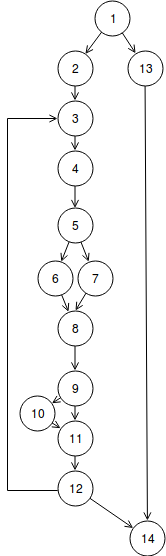
\includegraphics[width=.18\linewidth]{img/test-case/do_create}
  \caption{\emph{Flow graph} dari \emph{pseudocode} \emph{do\_create}}
  \label{cfg:create-vm-f}
\end{figure}

\noindent
\emph{Independent Path}

\begin{enumerate}
\item Jalur 1 : 1 - 13 - 14
\item Jalur 2 : 1 - 2 - 3 - 4 - 5 - 6 - 8 - 9 - 11 - 12 - 14
\item Jalur 3 : 1 - 2 - 3 - 4 - 5 - 7 - 8 - 9 - 11 - 12 - 14
\item Jalur 4 : 1 - 2 - 3 - 4 - 5 - 7 - 8 - 9 - 10 - 11 - 12 - 14
\item Jalur 5 : 1 - 2 - 3 - 4 - 5 - 7 - 8 - 9 - 10 - 11 - 12 - (for) - 12 - 14
\end{enumerate}

\begin{longtable}{|P{.06\textwidth}|P{.30\textwidth}|P{.30\textwidth}|P{.10\textwidth}|P{.08\textwidth}|}
  \caption{Pengujian \emph{integration} \emph{do\_create}} \label{jalur:create-vm-f} \\
  \hline
  \textbf{Jalur} & \textbf{Prosedur Uji} & \textbf{\emph{Expected Result}}
  & \textbf{\emph{Result}} & \textbf{Status} \\\hline
  %
  1 & Memberikan nilai \emph{raise exception} & Sistem menampilkan \emph{error log} dan
                               berhenti & \emph{As expected} & Valid \\\hline
                               %
  2 & 1)Memberikan nilai \emph{false} pada \emph{variable deploy\_env\_file}. \par\null\par
      2)Memberikan nilai lebih kecil dari 0 pada \emph{variable initialize}. \par\null\par
      3)Memberikan nilai \emph{false} pada kondisi \emph{deploy in initialize} bernilai \emph{false}
                                             & Sistem membuat
                                               \emph{virtual machine} tanpa \emph{env} dan tidak menjalankan
                                               \emph{sleep operation} & \emph{As expected} & Valid \\\hline
                                               %
  3 & 1)Memberikan nilai \emph{true} pada \emph{variable deploy\_env\_file} \emph{true}. \par\null\par
      2)Memberikan nilai lebih kecil dari 0 pada \emph{variable initialize}. \par\null\par
      3)Memberikan nilai \emph{false} pada kondisi \emph{deploy in initialize}
                                             & Sistem membuat
                                               \emph{virtual machine} dengan \emph{env} dan tidak menjalankan
                                               \emph{sleep operation} & \emph{As expected} & Valid \\\hline
                                               %
  4 & 1)Memberikan nilai \emph{true} pada \emph{variable deploy\_env\_file} \emph{true}. \par\null\par
      2)Memberikan nilai lebih besar dari 0 pada  \emph{variable initialize}. \par\null\par
      3)Memberikan nilai \emph{false} pada kondisi \emph{deploy in initialize}
                                             & Sistem membuat
                                               \emph{virtual machine} dengan \emph{env} dan menjalankan
                                               \emph{sleep operation} & \emph{As expected} & Valid \\\hline
                                               %
  5 & 1)Memberikan nilai \emph{true} pada \emph{variable deploy\_env\_file}. \par\null\par
      2)Memberikan nilai lebih besar dari 0 pada \emph{variable initialize}. \par\null\par
      3)Memberikan nilai \emph{true} pada kondisi \emph{deploy in initialize}
                                             & Sistem membuat
                                               \emph{virtual machine} dengan \emph{env} dan menjalankan
                                               \emph{sleep operation} & \emph{As expected} & Valid \\\hline
\end{longtable}

\subsubsection{\emph{Test Script} Untuk \emph{Automated Testing}}

\begin{code}
\begin{ignasicblock}[title=test\_do\_create,minted language=Python]
@pytest.mark.run(order=1)
def test_do_create(self):
    cwd = os.getcwd()
    deploy_init = orch.initialize(cwd + "/tests/neo.yml")
    orch.do_create(deploy_init)

    # check deployed vm
    vm_data = vm_lib.get_list()
    for vm in vm_data:
        if vm.name == 'unittest-vm':
            for network_name, network in vm.networks.items():
                assert network_name == 'unittest-network'
\end{ignasicblock}
\captionof{listing}{\emph{Test script} \emph{do\_create}}
\label{ts:create-vm-f}
\end{code}


\subsection{Kasus Uji NC3}

\subsubsection{Pengujian Unit \emph{get\_username}}

\begin{code}
\begin{ignasicblock}[title=get\_username,minted language=text]
procedure get_username()
    prompt username_input         (1)
    IF username_input <= 5 and    (2)
       username_input >= 255      (3)
       return username_input      (4)
    ELSE
       return false               (5)
    ENDIF                         (6)
end
\end{ignasicblock}
\captionof{listing}{\emph{Pseudocode} \emph{get\_username()}}
\label{pc:get_username}
\end{code}

\par\null\par
\noindent
\emph{Flow graph} yang dihasilkan dari \emph{pseudocode}
get\_username terlihat pada Gambar \ref{cfg:get_username}. \emph{Flow graph} tersebut memiliki
nilai \emph{cyclomatic complexity} V(G) = 3 \emph{regions} = 3.

\begin{figure}[H]
  \centering
  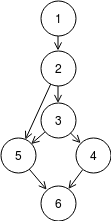
\includegraphics[width=.16\linewidth]{img/test-case/if-and-else}
  \caption{\emph{Flow graph} dari \emph{pseudocode} \emph{get\_username()}}
  \label{cfg:get_username}
\end{figure}

\noindent
\emph{Independent Path}

\begin{enumerate}
\item Jalur 1 : 1 - 2 - 5 - 6
\item Jalur 1 : 1 - 2 - 3 - 5 - 6
\item Jalur 1 : 1 - 2 - 3 - 4 - 6
\end{enumerate}

\newpage

\begin{longtable}{|P{.06\textwidth}|P{.30\textwidth}|P{.30\textwidth}|P{.10\textwidth}|P{.08\textwidth}|}
  \caption{Pengujian \emph{unit} \emph{get\_username}} \label{jalur:get_username}\\
  \hline
  \textbf{Jalur} & \textbf{Prosedur Uji} & \textbf{\emph{Expected Result}}
  & \textbf{\emph{Result}} & \textbf{Status} \\\hline
  %
  1 & Memberikan nilai \emph{false} pada kondisi ``username\_input <= 5'' & Sistem mengembalikan nilai
                                                                           \emph{false} & \emph{As expected} & Valid \\\hline
  2 & 1)Memberikan nilai \emph{true} pada kondisi ``username\_input <= 5'' \newline
      2)Memberikan nilai \emph{false} pada kondisi ``username\_input >= 255''
                                         & Sistem mengembalikan nilai \emph{false} & \emph{As expected} & Valid \\\hline
                                         %
  3 & 1)Memberikan nilai \emph{true} pada kondisi ``username\_input <= 5'' \newline
      2)Memberikan nilai \emph{true} pada kondisi ``username\_input >= 255''
                                         & Sistem mengembalikan nilai \emph{variable username\_input} & \emph{As expected} & Valid \\\hline
\end{longtable}

\subsubsection{Pengujian Unit \emph{get\_password}}

\begin{code}
\begin{ignasicblock}[title=get\_password,minted language=text]
procedure get_password()
    prompt password_input         (1)
    IF password_input <= 5 and    (2)
       password_input >= 255      (3)
       return password_input      (4)
    ELSE
       return false               (5)
    ENDIF                         (6)
end
\end{ignasicblock}
\captionof{listing}{\emph{Pseudocode} \emph{get\_password}}
\label{pc:get_password}
\end{code}

\noindent
\emph{Flow graph} yang dihasilkan dari \emph{pseudocode}
get\_password terlihat pada Gambar \ref{cfg:get_password}.
\emph{Flow graph} tersebut memiliki nilai \emph{cyclomatic complexity} V(G) = 3 \emph{regions} = 3.

\begin{figure}[H]
  \centering
  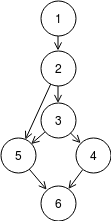
\includegraphics[width=.16\linewidth]{img/test-case/if-and-else}
  \caption{\emph{Flow graph} dari \emph{pseudocode} \emph{get\_password}}
  \label{cfg:get_password}
\end{figure}

\noindent
\emph{Independent Path}

\begin{enumerate}
\item Jalur 1 : 1 - 2 - 5 - 6
\item Jalur 1 : 1 - 2 - 3 - 5 - 6
\item Jalur 1 : 1 - 2 - 3 - 4 - 6
\end{enumerate}

\begin{longtable}{|P{.06\textwidth}|P{.30\textwidth}|P{.30\textwidth}|P{.10\textwidth}|P{.08\textwidth}|}
  \caption{Pengujian \emph{unit} \emph{get\_password}} \label{jalur:get_password} \\
  \hline
  \textbf{Jalur} & \textbf{Prosedur Uji} & \textbf{\emph{Expected Result}}
  & \textbf{\emph{Result}} & \textbf{Status} \\\hline
  %
  1 & Memberikan nilai \emph{false} pada kondisi ``password\_input <= 5'' & Sistem mengembalikan nilai
                                                                           \emph{false} & \emph{As expected} & Valid \\\hline
  2 & 1)Memberikan nilai \emph{true} pada kondisi ``password\_input <= 5'' \newline
      2)Memberikan nilai \emph{false} pada kondisi ``password\_input >= 255''
                                         & Sistem mengembalikan nilai \emph{false} & \emph{As expected} & Valid \\\hline
                                         %
  3 & 1)Memberikan nilai \emph{true} pada kondisi ``password\_input <= 5'' \newline
      2)Memberikan nilai \emph{true} pada kondisi ``password\_input >= 255''
                                         & Sistem mengembalikan nilai \emph{variable password\_input} & \emph{As expected} & Valid \\\hline
\end{longtable}

\subsubsection{Pengujian Unit \emph{generate\_session}}

\begin{code}
\begin{ignasicblock}[title=generate\_session,minted language=text]
procedure generate_session(password, password)
    sess = session with username and password   (1)
return sess
\end{ignasicblock}
\captionof{listing}{\emph{Pseudocode} \emph{generate\_session}}
\label{pc:generate_session}
\end{code}

\par\null\par
\noindent
\emph{Flow graph} yang dihasilkan dari \emph{pseudocode}
generate\_session terlihat pada Gambar \ref{cfg:generate_session}. \emph{Flow graph} tersebut memiliki nilai
\emph{cyclomatic complexity} V(G) = 2 \emph{regions} = 2.

\begin{figure}[H]
  \centering
  
\includegraphics[width=.06\linewidth]{img/test-case/1node}
  \caption{\emph{Flow graph} dari \emph{pseudocode} \emph{generate\_session}}
  \label{cfg:generate_session}
\end{figure}

\noindent
\emph{Independent Path}

\begin{enumerate}
\item 1 - 2 - 4
\item 1 - 3 - 4
\end{enumerate}


\begin{longtable}{|P{.06\textwidth}|P{.29\textwidth}|P{.29\textwidth}|P{.12\textwidth}|P{.08\textwidth}|}
  \caption{Pengujian \emph{unit} \emph{generate\_session}} \label{jalur:generate_session}\\
  \hline
  \textbf{Jalur} & \textbf{Prosedur Uji} & \textbf{\emph{Expected Result}}
  & \textbf{\emph{Result}} & \textbf{Status} \\\hline
  %
  1 & Menjalalankan \emph{generate\_session} & Sistem mengembalikan nilai dari \emph{variable sess}
  & \emph{As expected} & Valid \\\hline
  %
\end{longtable}

\subsubsection{Pengujian Integrasi \emph{do\_login}}

\begin{code}
\begin{ignasicblock}[title=do\_login,minted language=text]
procedure do_login()
    TRY                                     (1)
       username = get_username()            (2)
       password = get_password()
       generate_session(username, password)
       return true
    EXCEPT
       return false                         (3)
    ENDTRY                                  (4)
end
\end{ignasicblock}
\captionof{listing}{\emph{Pseudocode} \emph{do\_login}}
\label{pc:login}
\end{code}

\par\null\par
\noindent
\emph{Flow graph} yang dihasilkan dari \emph{pseudocode}
do\_login terlihat pada Gambar \ref{cfg:login}. \emph{Flow graph} tersebut memiliki nilai
\emph{cyclomatic complexity} V(G) = 2 \emph{regions} = 2.

\begin{figure}[H]
  \centering
  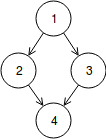
\includegraphics[width=.14\linewidth]{img/test-case/4node}
  \caption{\emph{Flow graph} dari \emph{pseudocode} \emph{do\_login}}
  \label{cfg:login}
\end{figure}

\noindent
\emph{Independent Path}

\begin{enumerate}
\item Jalur 1 : 1 - 2 - 4
\item Jalur 2 : 1 - 3 - 4
\end{enumerate}

\begin{longtable}{|P{.06\textwidth}|P{.30\textwidth}|P{.30\textwidth}|P{.10\textwidth}|P{.08\textwidth}|}
  \caption{Pengujian \emph{integration} \emph{do\_login}} \label{jalur:login}\\
  \hline
  \textbf{Jalur} & \textbf{Prosedur Uji} & \textbf{\emph{Expected Result}}
  & \textbf{\emph{Result}} & \textbf{Status} \\\hline
  %
  1 & Memberikan nilai  \emph{raise exception} & Sistem mengautentikasi pengguna & \emph{As expected} & Valid \\\hline
                                                 %
  2 & Tidak memberikan nilai  \emph{raise exception} & Sistem mengembalikan nilai \emph{false}
  & \emph{As expected} & Valid \\\hline
  %
\end{longtable}

\subsubsection{Pengujian \emph{input} \emph{do\_login} menggunakan \emph{equivalence partitioning}}

\emph{Method do\_login} meminta masukan kepada pengguna. Masukan
tersebut bertipe \emph{range}. Maka dilakukan teknik \emph{equivalence
partitioing} untuk memilih \emph{valid input} dan \emph{invalid input}
dalam metode pengujian \emph{black-box}.

\noindent
\emph{Equivalent Partitioning} test data

\begin{longtable}[c]{|l|p{4cm}|p{4cm}|}
  \caption{\emph{Equivalent Partitioning} \emph{do\_login}} \label{tc:login-eq} \\
  \hline
  \textbf{Input} & \textbf{\emph{Valid Class}} & \textbf{\emph{Invalid Class}}\\\hline
  %
  Nilai \emph{username}  & Segala karakter dengan jumlah batas minimum
                           5 dan maksimum 255
                                               & Segala karakter dengan jumlah kurang dari 5
                                                 dan lebih dari 255 \\\hline
                                                 %
  Nilai \emph{password}  & Segala karakter dengan jumlah batas minimum
                           5 dan maksimum 255
                                               & Segala karakter dengan jumlah kurang dari 5
                                                 dan lebih dari 255 \\\hline
                                                 %
\end{longtable}

\noindent
Pada teknik \emph{equivalence partitioning} \emph{argument} nilai
\emph{username} dan \emph{password} merupakan tipe \emph{range}. Maka
didaptkan satu data \emph{valid} dan dua data \emph{invalid}.

\begin{itemize}
\item Nilai \emph{username}
  \begin{itemize}
  \item Kasus uji \emph{valid} : `azzamsa'
  \item Kasus uji \emph{invalid}  : [karakter dengan jumlah 2], [karakter dengan jumlah 260]
  \end{itemize}
\item Nilai \emph{password}
  \begin{itemize}
  \item Kasus uji \emph{valid} : `foobar'
  \item Kasus uji \emph{invalid}  : [karakter dengan jumlah 2], [karakter dengan jumlah 260]
  \end{itemize}
\end{itemize}

\begin{longtable}{|P{.06\textwidth}|P{.30\textwidth}|P{.30\textwidth}|P{.10\textwidth}|P{.08\textwidth}|}
  \caption{Pengujian  \emph{input} \emph{do\_login} dengan teknik \emph{equivalence partitioning}} \label{jalur:login-eq}\\
  \hline
  \textbf{No} & \textbf{Prosedur Uji} & \textbf{\emph{Expected Result}} & \textbf{\emph{Result}} & \textbf{Status} \\\hline
  %
  1 & 1)Memberikan nilai \emph{valid} `azzamsa' pada \emph{username} \newline
      2)Memberikan nilai \emph{valid} `foobar' pada \emph{password}
                                      & Autentikasi pengguna berhasil
                                                                        & \emph{As expected} & Valid \\\hline
                                                                        %
  2 & 1)Memberikan nilai \emph{invalid} [karakter dengan jumlah 2] pada \emph{username} \newline
      2)Memberikan nilai \emph{invalid} [karakter dengan jumlah 2] pada \emph{password}
                                      & Autentikasi pengguna gagal
                                                                        & \emph{As expected} & Valid \\\hline
                                                                        %
  3 & 1)Memberikan nilai \emph{invalid} [karakter dengan jumlah 260] pada \emph{username} \newline
      2)Memberikan nilai \emph{invalid} [karakter dengan jumlah 260] pada \emph{password}
                                      & Autentikasi pengguna gagal
                                                                        & \emph{As expected} & Valid \\\hline
                                                                        %
  %
\end{longtable}

\subsubsection{Pengujian \emph{Input} \emph{do\_login} Menggunakan \emph{Boundary Value Analysis}}

\emph{Method do\_login} meminta masukan kepada pengguna. Masukan
tersebut bertipe \emph{range}. Maka dilakukan teknik \emph{boundary
  value analysis} untuk memilih \emph{input} yang berada pada daerah
\emph{boundary} dalam metode pengujian \emph{black-box}. \\

\noindent
\emph{Boundary Value Analysis} test data

\newpage

\begin{longtable}[c]{|l|p{7cm}|}
  \caption{\emph{Boundary Value} \emph{login}} \label{tc:login-bva}\\
  \hline
  \textbf{Input} & \textbf{\emph{Boundary Value}}\\\hline
  %
  Nilai \emph{username}  & Jumlah karakter satu tingkat dibawah batas minimum dan
                           satu tingkat diatas maksimum\\\hline
                           %
  Nilai \emph{password}  & Jumlah karakter satu tingkat dibawah batas minimum dan
                           satu tingkat diatas maksimum\\\hline
                           %
\end{longtable}

\noindent
Pada teknik \emph{boundary value analysis}. Nilai \emph{username} dan
\emph{password} merupakan tipe \emph{range}. Maka kasus uji didapatkan
dari satu nilai dibawah batas minimum dan satu nilai diatas batas
maksimum.

\begin{itemize}
\item Nilai \emph{boundary}  untuk \emph{username}
  \begin{itemize}
  \item Satu nilai dibawah minimum : [karakter dengan jumlah 4]
  \item Satu nilai diatas maksimum  : [karakter dengan jumlah 6]
  \end{itemize}
\item Nilai \emph{boundary} untuk \emph{password}
  \begin{itemize}
  \item Satu nilai dibawah minimum : [karakter dengan jumlah 254]
  \item Satu nilai diatas maksimum  : [karakter dengan jumlah 256]
  \end{itemize}
\end{itemize}


\begin{longtable}{|P{.06\textwidth}|P{.30\textwidth}|P{.30\textwidth}|P{.10\textwidth}|P{.08\textwidth}|}
  \caption{Pengujian  \emph{input} \emph{do\_login} dengan teknik \emph{boundary value analysis}} \label{jalur:login-bva}\\
  \hline
  \textbf{No} & \textbf{Prosedur Uji} & \textbf{\emph{Expected Result}} & \textbf{\emph{Result}} & \textbf{Status} \\\hline
  %
  1 & 1)Memberikan nilai \emph{invalid} [karakter dengan jumlah 4] pada \emph{username} \newline
      2)Memberikan nilai \emph{invalid} [karakter dengan jumlah 254] pada \emph{password}
                                      & Autentikasi pengguna gagal
                                                                        & \emph{As expected} & Valid \\\hline
                                                                        %
  2 & 1)Memberikan nilai \emph{invalid} [karakter dengan jumlah 6] pada \emph{username} \newline
      2)Memberikan nilai \emph{invalid} [karakter dengan jumlah 256] pada \emph{password}
                                      & Autentikasi pengguna gagal
                                                                        & \emph{As expected} & Valid \\\hline
                                                                        %
\end{longtable}


\subsubsection{\emph{Test Script} Untuk \emph{Automated Testing}}

\begin{code}
\begin{ignasicblock}[title=test\_do\_login,minted language=Python]
@pytest.mark.run(order=0)
def test_do_login(self, monkeypatch):
    login.load_env_file()
    username = os.environ.get('OS_USERNAME')
    passwd = os.environ.get('OS_PASSWORD')
    # give value to input() prompt
    monkeypatch.setattr('builtins.input', lambda x: username)
    monkeypatch.setattr('getpass.getpass', lambda x: passwd)
    # return True is login succeed
    output = login.do_login()
    assert output == True
\end{ignasicblock}
\captionof{listing}{\emph{Test script} utnuk \emph{do\_login}}
\label{ts:login}
\end{code}

\subsection{Kasus Uji NC4}

\subsubsection{Pengujian Unit \emph{check\_session}}

\begin{code}
\begin{ignasicblock}[title=check\_session,minted language=text]
procedure check_session()
    return is_session_pkl_exist (1)
end
\end{ignasicblock}
\captionof{listing}{\emph{Pseudocode} \emph{check\_session}}
\label{pc:check_session}
\end{code}

\par\null\par
\noindent
\emph{Flow graph} yang dihasilkan dari \emph{pseudocode}
check\_session terlihat pada Gambar \ref{cfg:check_session}.
\emph{Flow graph} tersebut memiliki nilai \emph{cyclomatic complexity} V(G) = 1 \emph{region} = 1.

\begin{figure}[H]
  \centering
  
\includegraphics[width=.06\linewidth]{img/test-case/1node}
  \caption{\emph{Flow graph} dari \emph{pseudocode} \emph{check\_session}}
  \label{cfg:check_session}
\end{figure}

\noindent
\emph{Independent Path}

\begin{enumerate}
\item Jalur 1 : 1
\end{enumerate}

\begin{longtable}{|P{.06\textwidth}|P{.30\textwidth}|P{.30\textwidth}|P{.10\textwidth}|P{.08\textwidth}|}
  \caption{Pengujian \emph{unit} \emph{check\_session}} \label{jalur:check_session} \\
  \hline
  \textbf{Jalur} & \textbf{Prosedur Uji} & \textbf{\emph{Expected Result}}
  & \textbf{\emph{Result}} & \textbf{Status} \\\hline
  %
  1 & Menjalankan \emph{check\_session} & Sistem akan mengembalikan nilai dari fungsi
                                          \emph{is\_session\_pkl\_exist} & \emph{As expected} & Valid \\\hline
                                          %
\end{longtable}

\subsubsection{Pengujian integrasi \emph{do\_logout}}

\begin{code}
\begin{ignasicblock}[title=do\_logout,minted language=text]
procedure do_logout()
    IF check_session()
        remove login_data     (1)
    ENDIF
end
\end{ignasicblock}
\captionof{listing}{\emph{Pseudocode} \emph{do\_logout}}
\label{pc:do_logout}
\end{code}

\par\null\par
\noindent
\emph{Flow graph} yang dihasilkan dari \emph{pseudocode}
do\_logout terlihat pada Gambar \ref{cfg:do_logout}. \emph{Flow graph} tersebut memiliki
nilai \emph{cyclomatic complexity} V(G) = 1 \emph{region} = 1.

\begin{figure}[H]
  \centering
  
\includegraphics[width=.06\linewidth]{img/test-case/1node}
  \caption{\emph{Flow graph} dari \emph{pseudocode} \emph{do\_logout}}
  \label{cfg:do_logout}
\end{figure}

\newpage

\noindent
\emph{Independent Path}

\begin{enumerate}
\item Jalur 1 : 1
\end{enumerate}

\begin{longtable}{|P{.06\textwidth}|P{.30\textwidth}|P{.30\textwidth}|P{.10\textwidth}|P{.08\textwidth}|}
  \caption{Pengujian \emph{integration} \emph{do\_logout}} \label{jalur:do_logout}\\
  \hline
  \textbf{Jalur} & \textbf{Prosedur Uji} & \textbf{\emph{Expected Result}}
  & \textbf{\emph{Result}} & \textbf{Status} \\\hline
  %
  1 & Memberikan nilai \emph{true} pada nilai \emph{return method check\_session}
                                             & Sistem menghapus
                                               data autentikasi & \emph{As expected} & Valid \\\hline
                                               %
\end{longtable}

\subsubsection{\emph{Test Script} Untuk \emph{Automated Testing}}

\begin{code}
\begin{ignasicblock}[title=test\_do\_logout,minted language=Python]
@pytest.mark.run(order=-1)
def test_do_logout(self):
    login.do_logout()
    # session removed if logout succeed
    output = login.check_session()
    assert output == False
\end{ignasicblock}
\captionof{listing}{\emph{test script} \emph{logout}}
\label{ts:do_logout}
\end{code}


\subsection{Kasus Uji NC5}

\subsubsection{Pengujian Unit \emph{get\_heat\_client}}

\noindent
Pengujian \emph{unit} pada \emph{method get\_heat\_client} telah
dilakukan sebelumnya pada Tabel ~\ref{cfg:get_heat_client}

\subsubsection{Pengujian Integrasi \emph{get\_stack\_list}}

\begin{code}
\begin{ignasicblock}[title=get\_stack\_list,minted language=text]
procedure get_stack_list()
    h_client = get_heat_client()
    stack_list = h_client CALL heat_stack_value  (1)
    return stack_list
end
\end{ignasicblock}
\captionof{listing}{\emph{Pseudocode} \emph{get\_list}}
\label{pc:get_list}
\end{code}

\par\null\par
\noindent
\emph{Flow graph} yang dihasilkan dari \emph{pseudocode}
get\_list terlihat pada Gambar \ref{cfg:get_list}. \emph{Flow graph} tersebut memiliki
nilai \emph{cyclomatic complexity} V(G) = 1 \emph{region} = 1.

\begin{figure}[H]
  \centering
  
\includegraphics[width=.06\linewidth]{img/test-case/1node}
  \caption{\emph{Flow graph} dari \emph{pseudocode} \emph{get\_list}}
  \label{cfg:get_list}
\end{figure}

\noindent
\emph{Independent Path}

\begin{enumerate}
\item Jalur 1 : 1
\end{enumerate}

\begin{longtable}{|P{.06\textwidth}|P{.30\textwidth}|P{.30\textwidth}|P{.10\textwidth}|P{.08\textwidth}|}
  \hline
  \textbf{Jalur} & \textbf{Prosedur Uji} & \textbf{\emph{Expected Result}}
  & \textbf{\emph{Result}} & \textbf{Status} \\\hline
  %
  1 & Menjalankan \emph{get\_list}  & Sistem akan melempar nilai \emph{variable data\_stack}
  & \emph{As expected} & Valid \\\hline
  %
  \caption{Pengujian \emph{unit} \emph{get\_list}}
  \label{jalur:get_list}
\end{longtable}


\subsubsection{\emph{Test Script} Untuk \emph{Automated Testing}}


\begin{code}
\begin{ignasicblock}[title=test\_ls\_stack,minted language=Python]
def test_ls_stack(self):
        with pytest.raises(SystemExit):
            a = Ls({'<command>': 'ls'}, 'stack')
            a.execute()
\end{ignasicblock}
\captionof{listing}{\emph{Test script} \emph{get\_stack\_list}}
\label{ts:ls-stack}
\end{code}

\subsection{Kasus Uji NC6}

\subsubsection{Pengujian Unit \emph{get\_neutron\_client}}

Pengujian unit dilakukan pada \emph{method get\_neutron\_client}
secara terisolasi dan sebagai \emph{stand-alone program}.  Maka
dilakukan \emph{mocking} pada \emph{method load\_dumped\_session} dan
\emph{neutron\_client}.

\begin{code}
\begin{ignasicblock}[title=get\_neutron\_client,minted language=text]
procedure get_neutron_client()
    IF not session:
        session = load_dumped_session()   (1)
        neutron = neutron_client()
        return neutron
    ENDIF
end
\end{ignasicblock}
\captionof{listing}{\emph{Pseudocode} \emph{get\_neutron\_client}}
\label{pc:get_neutron_client}
\end{code}

\par\null\par
\noindent
\emph{Flow graph} yang dihasilkan dari \emph{pseudocode}
get\_neutron\_client terlihat pada Gambar \ref{cfg:get_neutron_client}.
\emph{Flow graph} tersebut memiliki nilai \emph{cyclomatic complexity} V(G) = 1 \emph{regions} = 1.

\begin{figure}[H]
  \centering
  
\includegraphics[width=.06\linewidth]{img/test-case/1node}
  \caption{\emph{Flow graph} dari \emph{pseudocode} \emph{get\_neutron\_client}}
  \label{cfg:get_neutron_client}
\end{figure}

\noindent
\emph{Independent Path}

\begin{enumerate}
\item Jalur 1 : 1
\end{enumerate}

\begin{longtable}{|P{.06\textwidth}|P{.30\textwidth}|P{.30\textwidth}|P{.10\textwidth}|P{.08\textwidth}|}
  \caption{Pengujian \emph{unit} \emph{get\_neutron\_client}} \label{jalur:get_neutron_client}\\
  \hline
  \textbf{Jalur} & \textbf{Prosedur Uji} & \textbf{\emph{Expected Result}}
  & \textbf{\emph{Result}} & \textbf{Status} \\\hline
  %
  1 & Memberikan nilai \emph{true} pada  \emph{variable session}
                                             & Sistem mengembalikan nilai \emph{variable neutron}
  & \emph{As expected} & Valid \\\hline
  %
\end{longtable}

\subsubsection{Pengujian Unit \emph{get\_network\_list}}

Pengujian unit dilakukan pada \emph{method get\_list} secara
terisolasi dan sebagai \emph{stand-alone program}.  Maka dilakukan
\emph{mocking} pada \emph{method list\_networks}.

\begin{code}
\begin{ignasicblock}[title=get\_network\_list,minted language=text]
procedure get_network_list()
    TRY                                          (1)
        n_client = get_neutron_client()
        networks = n_client CALL list_networks() (2)
        return networks
    EXCEPT
        show_error_log                           (3)
    ENDTRY                                       (4)
end
\end{ignasicblock}
\captionof{listing}{\emph{Pseudocode} \emph{get\_network\_list}}
\label{pc:get_list_network}
\end{code}

\par\null\par
\noindent
\emph{Flow graph} yang dihasilkan dari \emph{pseudocode}
get\_network\_list terlihat pada Gambar \ref{cfg:get_list_network}.
\emph{Flow graph} tersebut memiliki nilai \emph{cyclomatic complexity} V(G) = 2 \emph{regions} = 2.

\begin{figure}[H]
  \centering
  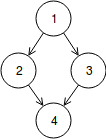
\includegraphics[width=.14\linewidth]{img/test-case/4node}
  \caption{\emph{Flow graph} dari \emph{pseudocode} \emph{get\_network\_list}}
  \label{cfg:get_list_network}
\end{figure}

\noindent
\emph{Independent Path}~\ref{cfg:get_list_network}

\begin{enumerate}
\item Jalur 1 : 1 - 2 - 4
\item Jalur 2 : 1 - 3 - 4
\end{enumerate}


\begin{longtable}{|P{.05\textwidth}|P{.30\textwidth}|P{.30\textwidth}|P{.10\textwidth}|P{.08\textwidth}|}
  \caption{Pengujian \emph{unit} \emph{get\_network\_list}} \label{jalur:get_list_network}\\
  \hline
  \textbf{Jalur} & \textbf{Prosedur Uji} & \textbf{\emph{Expected Result}}
  & \textbf{\emph{Result}} & \textbf{Status} \\\hline
  %
  1 & Melakukan \emph{raise exception}  & Sistem mengembalikan nilai
                                          \emph{variable network} & \emph{As expected} & Valid \\\hline
  %
  2 & Tidak melakukan \emph{raise exception} & Sistem menampilkan \emph{error log} dan
                                               berhenti & \emph{As expected} & Valid \\\hline
  %
\end{longtable}

\subsubsection{Pengujian Integrasi \emph{list\_network}}

Pengujian \emph{unit} dilakukan pada \emph{method list\_network}
secara terisolasi dan sebagai \emph{stand-alone program}. Maka
dilakukan \emph{mocking} pada \emph{method get\_network\_list}.

\begin{code}
\begin{ignasicblock}[title=list\_network,minted language=text]
procedure list_network()
    network_list = get_network_list()     (1)
    IF network_list == 0                  (2)
        print `no data'                   (3)
    ELSE
        print network_list                (4)
    ENDIF                                 (5)
end
\end{ignasicblock}
\captionof{listing}{\emph{Pseudocode} \emph{list\_network}}
\label{pc:ls-network}
\end{code}

\par\null\par
\noindent
\emph{Flow graph} yang dihasilkan dari \emph{pseudocode}
list\_network terlihat pada Gambar \ref{cfg:list_network}.
\emph{Flow graph} tersebut memiliki nilai \emph{cyclomatic complexity} V(G) = 2 \emph{regions} = 2.

\begin{figure}[H]
  \centering
  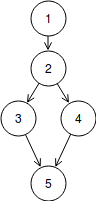
\includegraphics[width=.15\linewidth]{img/test-case/is_current_env}
  \caption{\emph{Flow graph} dari \emph{pseudocode} \emph{ist\_network}}
  \label{cfg:list_network}
\end{figure}

\noindent
\emph{Independent Path}

\begin{enumerate}
\item Jalur 1 : 1 - 2 - 3 - 5
\item Jalur 1 : 1 - 2 - 4 - 5
\end{enumerate}

\newpage

\begin{longtable}{|P{.06\textwidth}|P{.30\textwidth}|P{.30\textwidth}|P{.10\textwidth}|P{.08\textwidth}|}
  \caption{Pengujian \emph{integration} \emph{list\_network}} \label{jalur:ls-network}\\
  \hline
  \textbf{Jalur} & \textbf{Prosedur Uji} & \textbf{\emph{Expected Result}}
  & \textbf{\emph{Result}} & \textbf{Status} \\\hline
  %
  1 & Memberikan nilai 0 pada \emph{variable network\_list}
                                             & Sistem akan menampilan pesan
                                               `no data' & \emph{As expected} & Valid \\\hline
  %
  2 & Memberikan nilai 1 pada \emph{variable network\_list}  & Sistem akan menampilkan daftar \emph{network} & \emph{As expected} & Valid \\\hline
  %
\end{longtable}

\subsubsection{\emph{Test Script} Untuk \emph{Automated Testing}}

\begin{code}
\begin{ignasicblock}[title=test\_ls\_net,minted language=Python]
def test_ls_net(self):
        with pytest.raises(SystemExit):
            a = Ls({'<command>': 'ls'}, 'network')
            a.execute()
\end{ignasicblock}
\captionof{listing}{\emph{Test script} \emph{ls network}}
\label{ts:ls-network}
\end{code}

\subsection{Kasus Uji NC7}

\subsubsection{Pengujian Unit \emph{get\_nova\_client}}

Pengujian \emph{unit} dilakukan pada \emph{method get\_nova\_client}
secara terisolasi dan sebagai \emph{stand-alone program}. Maka
dilakukan \emph{mocking} pada \emph{method nova\_client}.

\begin{code}
\begin{ignasicblock}[title=get\_nova\_client,minted language=text]
procedure get_nova_client(session)
    IF not session:
        compute = nova_client()   (1)
    return compute
    ENDIF
end
\end{ignasicblock}
\captionof{listing}{\emph{Pseudocode} \emph{get\_nova\_client}}
\label{pc:get_nova_client}
\end{code}

\par\null\par
\noindent
\emph{Flow graph} yang dihasilkan dari \emph{pseudocode}
get\_nova\_client terlihat pada Gambar \ref{cfg:get_nova_client}.
\emph{Flow graph} tersebut memiliki nilai \emph{cyclomatic complexity} V(G) = 1 \emph{region} = 1.

\begin{figure}[H]
  \centering
  
\includegraphics[width=.06\linewidth]{img/test-case/1node}
  \caption{\emph{Flow graph} dari \emph{pseudocode} \emph{get\_nova\_client}}
  \label{cfg:get_nova_client}
\end{figure}

\noindent
\emph{Independent Path}

\begin{enumerate}
\item Jalur 1 : 1
\end{enumerate}


\begin{longtable}{|P{.06\textwidth}|P{.30\textwidth}|P{.30\textwidth}|P{.10\textwidth}|P{.08\textwidth}|}
  \caption{Pengujian \emph{unit} \emph{get\_nova\_client}} \label{jalur:get_nova_client}\\
  \hline
  \textbf{Jalur} & \textbf{Prosedur Uji} & \textbf{\emph{Expected Result}}
  & \textbf{\emph{Result}} & \textbf{Status} \\\hline
  %
  1 & Menjalankan \emph{get\_nova\_client} & Sistem mengembalikan nilai
                                             \emph{variable compute} & \emph{As expected} & Valid \\\hline
  %
\end{longtable}

\subsubsection{Pengujian Integrasi \emph{do\_delete}}

\begin{code}
\begin{ignasicblock}[title=do\_delete,minted language=text]
procedure do_delete(instance_id, session)    (1)
    initialize compute = get_nova_client()
    compute_delete(instnce_id)
end
\end{ignasicblock}
\captionof{listing}{\emph{Pseudocode} \emph{do\_delete}}
\label{pc:rm_vm}
\end{code}

\par\null\par
\noindent
\emph{Flow graph} yang dihasilkan dari \emph{pseudocode}
do\_delete terlihat pada Gambar \ref{cfg:rm_vm}.
\emph{Flow graph} tersebut memiliki nilai \emph{cyclomatic complexity} V(G) = 1 \emph{region} = 1.

\begin{figure}[H]
  \centering
  
\includegraphics[width=.06\linewidth]{img/test-case/1node}
  \caption{\emph{Flow graph} dari \emph{pseudocode} \emph{do\_delete}}
  \label{cfg:rm_vm}
\end{figure}

\noindent
\emph{Independent Path}

\begin{enumerate}
\item Jalur 1 : 1
\end{enumerate}


\begin{longtable}{|P{.06\textwidth}|P{.30\textwidth}|P{.30\textwidth}|P{.10\textwidth}|P{.08\textwidth}|}
  \caption{Pengujian \emph{integration} \emph{do\_delete}} \label{jalur:rm-vm}\\
  \hline
  \textbf{Jalur} & \textbf{Prosedur Uji} & \textbf{\emph{Expected Result}}
  & \textbf{\emph{Result}} & \textbf{Status} \\\hline
  %
  1 & Menjalankan \emph{do\_delete} & Sistem menghapus \emph{virtual machine} & \emph{As expected} & Valid \\\hline
  %
\end{longtable}

\subsubsection{\emph{Test Script} Untuk \emph{Automated Testing}}

\begin{code}
\begin{ignasicblock}[title=test\_do\_delete\_vm,minted language=Python]
@pytest.mark.run(order=-2)
    def test_do_delete_vm(self):
        # wait until successfully created
        vm_status = ''
        while vm_status != 'ACTIVE':
            # get 'unittest-vm' id
            vm_data = vm_lib.get_list()
            for vm in vm_data:
                if vm.name == 'unittest-vm':
                    vm_status = vm.status
                    instance_id = vm.id
                    vm_name = vm.name
            time.sleep(2)
            print('waiting until vm activated ...')

        vm_lib.do_delete(instance_id)
        print(vm_name + ' with id ' + instance_id + ' deleted')

        # wait until successfully deleted
        while 'unittest' in vm_data:
            vm_data = vm_lib.get_list()
            time.sleep(2)
            print('waiting until vm fully deleted ...')

        assert 'unittest-vm' not in vm_data
\end{ignasicblock}
\captionof{listing}{\emph{Test script} \emph{do\_delete}}
\label{ts:rm-vm}
\end{code}

\subsection{Kasus Uji NC8}

\subsubsection{Pengujian Unit \emph{get\_heat\_client}}

Pengujian \emph{unit} untuk \emph{get\_heat\_client} telah dilakukan sebelumnya
pada Tabel ~\ref{jalur:get_heat_client}.

\subsubsection{Pengujian Integrasi \emph{do\_delete}}

\begin{code}
\begin{ignasicblock}[title=do\_delete,minted language=text]
procudure do_delete(stack_name)
    TRY                                   (1)
        delete stack_name                 (2)
        return true
    EXCEPT
        return false                      (3)
    ENDTRY                                (4)
end
    \end{ignasicblock}
  \captionof{listing}{\emph{Pseudocode} \emph{do\_delete}}
  \label{pc:rm_stack}
\end{code}

\par\null\par
\noindent
\emph{Flow graph} yang dihasilkan dari \emph{pseudocode}
do\_delete terlihat pada Gambar \ref{cfg:rm_stack}.
\emph{Flow graph} tersebut memiliki nilai \emph{cyclomatic complexity} V(G) = 2 \emph{regions} = 2.

\begin{figure}[H]
  \centering
  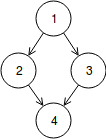
\includegraphics[width=.14\linewidth]{img/test-case/4node}
  \caption{\emph{Flow graph} dari \emph{pseudocode} \emph{do\_delete}}
  \label{cfg:rm_stack}
\end{figure}

\noindent
\emph{Independent Path}

\begin{enumerate}
\item Jalur 1 : 1 - 2 - 4
\item Jalur 2 : 1 - 3 - 4
\end{enumerate}

\newpage

\begin{longtable}{|P{.06\textwidth}|P{.30\textwidth}|P{.30\textwidth}|P{.10\textwidth}|P{.08\textwidth}|}
  \caption{Pengujian \emph{integration} \emph{do\_delete}} \label{jalur:rm-stack}\\
  \hline
  \textbf{Jalur} & \textbf{Prosedur Uji} & \textbf{\emph{Expected Result}}
  & \textbf{\emph{Result}} & \textbf{Status} \\\hline
  %
  1 & Tidak melakukan  \emph{raise exception} & \emph{Stack} berhasil dihapus
                                          \emph{true} & \emph{As expected} & Valid \\\hline
  %
  2 & Melakukan  \emph{raise exception} & \emph{Stack} tidak terhapus & \emph{As expected} & Valid \\\hline
  %
\end{longtable}

\subsubsection{\emph{Test Script} Untuk \emph{Automated Testing}}

\begin{code}
\begin{ignasicblock}[title=test\_do\_delete\_stack,minted language=Python]
@pytest.mark.run(order=-2)
def test_do_delete_stack(self):
    # wait until successfully created
    vm_status = ''
    while vm_status != 'ACTIVE':
        # get 'unittest-vm' id
        vm_data = vm_lib.get_list()
        for vm in vm_data:
            if vm.name == 'unittest-vm':
                vm_status = vm.status
                instance_id = vm.id
                vm_name = vm.name
        time.sleep(2)
        print('waiting until vm activated ...')

    orch.do_delete('unittest-network')
    orch.do_delete('unittest-key')
    print(vm_name + ' with id ' + instance_id + ' deleted')

    # wait until successfully deleted
    while 'unittest' in vm_data:
        vm_data = vm_lib.get_list()
        time.sleep(2)
        print('waiting until vm fully deleted ...')

    assert 'unittest-vm' not in vm_data
\end{ignasicblock}
  \captionof{listing}{\emph{Test script} \emph{do\_delete}}
  \label{ts:rm_stack}
\end{code}

\subsection{Kasus Uji NC9}

\subsubsection{Pengujian Unit \emph{get\_heat\_client}}

\noindent
Pengujian \emph{unit} untuk \emph{method get\_heat\_client} telah dilakukan sebelumnya
pada Tabel~\ref{jalur:get_heat_client}

\subsubsection{Pengujian Unit \emph{yaml\_parser}}

\noindent
Pengujian \emph{unit} untuk \emph{method yaml\_parser} telah dilakukan sebelumnya
pada Tabel~\ref{jalur:yaml_parser}.

\subsubsection{Pengujian Integrasi \emph{do\_update}}

\begin{code}
\begin{ignasicblock}[title=do\_update,minted language=text]
procedure do_update(initialize)
    TRY                                               (1)
        initialize heat = get_heat_client()           (2)
        FOR deploy in initialize:                     (3)
            deploy_init_file = deploy_dir             (4)
            deploy_file = yaml_parser(deploy_init_file)
            deploy_template = deploy_file
            deploy_name = deploy_project
            IF not deploy_env_file                    (5)
              update_stack_without_env                (6)
            ELSE
              update_stack_with_env                   (7)
            ENDIF                                     (8)
            IF initialize > 0                         (9)
              sleep operation                         (10)
            ENDIF                                     (11)
        ENDFOR                                        (12)
    EXCEPT
       show_error_log                                 (13)
    ENDTRY                                            (14)
end
\end{ignasicblock}
  \captionof{listing}{\emph{Pseudocode} \emph{do\_update}}
  \label{pc:update}
\end{code}

\par\null\par
\noindent
\emph{Flow graph} yang dihasilkan dari \emph{pseudocode}
do\_update terlihat pada Gambar \ref{cfg:update}.
\emph{Flow graph} tersebut memiliki nilai \emph{cyclomatic complexity} V(G) = 5 \emph{regions} = 5.

\begin{figure}[H]
  \centering
  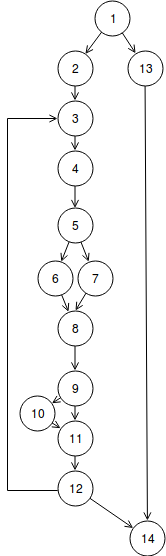
\includegraphics[width=.18\linewidth]{img/test-case/do_create} % sama cfgnya
  \caption{\emph{Flow graph} dari \emph{pseudocode} \emph{do\_update}}
  \label{cfg:update}
\end{figure}

\noindent
\emph{Independent Path}

\begin{enumerate}
\item Jalur 1 : 1 - 13 - 14
\item Jalur 2 : 1 - 2 - 3 - 4 - 5 - 6 - 8 - 9 - 11 - 12 - 14
\item Jalur 3 : 1 - 2 - 3 - 4 - 5 - 7 - 8 - 9 - 11 - 12 - 14
\item Jalur 4 : 1 - 2 - 3 - 4 - 5 - 7 - 8 - 9 - 10 - 11 - 12 - 14
\item Jalur 5 : 1 - 2 - 3 - 4 - 5 - 7 - 8 - 9 - 10 - 11 - 12 - (for) - 12 - 14
\end{enumerate}


\begin{longtable}{|P{.06\textwidth}|P{.30\textwidth}|P{.30\textwidth}|P{.10\textwidth}|P{.08\textwidth}|}
  \caption{Pengujian \emph{integration} \emph{do\_update}} \label{jalur:update}\\
  \hline
  \textbf{Jalur} & \textbf{Prosedur Uji} & \textbf{\emph{Expected Result}}
  & \textbf{\emph{Result}} & \textbf{Status} \\\hline
  %
  1 & Melakukan\emph{raise exception} & Sistem menampilkan \emph{error log} dan
                               berhenti & \emph{As expected} & Valid \\\hline
                               %
  2 & 1)Memberikan nilai \emph{false} pada \emph{variable deploy\_env\_file} \par\null\par
      2)Memberikan nilai lebih kecil dari 0 pada \emph{variable initialize} \par\null\par
      3)Memberikan nilai \emph{false} pada kondisi \emph{deploy in initialize}
                                             & Sistem memperbarui
                                               \emph{virtual machine} tanpa \emph{env} dan tidak menjalankan
                                     \emph{sleep operation} & \emph{As expected} & Valid \\\hline
                                               %
  3 & 1)Memberikan nilai \emph{true} pada \emph{variable deploy\_env\_file} \par\null\par
      2)Memberikan nilai lebih kecil dari 0 pada \emph{variable initialize} \par\null\par
      3)Memberikan nilai \emph{false} pada kondisi \emph{deploy in initialize}
                                             & Sistem memperbarui
                                               \emph{virtual machine} dengan \emph{env} dan tidak menjalankan
                                               \emph{sleep operation} & \emph{As expected} & Valid \\\hline
                                               %
  4 & 1)Memberikan nilai \emph{true} pada \emph{variable deploy\_env\_file} \par\null\par
      2)Memberikan nilai lebih besar dari 0 pada \emph{variable initialize} \par\null\par
      3)Memberikan nilai \emph{false} pada kondisi \emph{deploy in initialize}
                                             & Sistem memperbarui
                                               \emph{virtual machine} dengan \emph{env} dan menjalankan
                                               \emph{sleep operation} & \emph{As expected} & Valid \\\hline
                                               %
  5 & 1)Memberikan nilai \emph{true} pada \emph{variable deploy\_env\_file} \par\null\par
      2)Memberikan nilai lebih besar dari 0 pada \emph{variable initialize} \par\null\par
      3)Memberikan nilai \emph{true} pada kondisi \emph{deploy in initialize}
                                             & Sistem memperbarui
                                               \emph{virtual machine} dengan \emph{env} dan menjalankan
                                               \emph{sleep operation} & \emph{As expected} & Valid \\\hline
\end{longtable}


\subsubsection{\emph{Test Script} Untuk \emph{Automated Testing}}

\begin{code}
\begin{ignasicblock}[title=test\_do\_update,minted language=Python]
    @pytest.mark.run(order=2)
    def test_do_update(self):
        cwd = os.getcwd()

        # wait until last vm successfully created
        vm_status = ''
        while vm_status != 'ACTIVE':
            # get 'unittest-vm' id
            vm_data = vm_lib.get_list()
            for vm in vm_data:
                if vm.name == 'unittest-vm':
                    vm_status = vm.status
                    vm_name = vm.name
            time.sleep(2)
            print('waiting until vm activated ...')

        a = Update({'<args>': ['-f', 'tests/neo2.yml'],
                    '<command>': 'update'}, '-f', 'tests/neo2.yml')
        a.execute()
        print(vm_name + ' updated')

        # wait until successfully updated
        updated_status = None
        while updated_status == None:
            vm_data = orch.get_list()
            for vm in vm_data:
                if "unittest-vm" in vm:
                    updated_status = vm[4]
            time.sleep(2)
            print('waiting until vm fully updated ...')

        assert updated_status != None
\end{ignasicblock}
  \captionof{listing}{\emph{Test script} \emph{do\_update}}
  \label{ts:update}
\end{code}

\subsection{Kasus Uji NC10}

\subsubsection{Pengujian Integrasi \emph{show\_help}}

\begin{code}
\begin{ignasicblock}[title=show\_help,minted language=text]
procudure show_help()
    print help       (1)
end
\end{ignasicblock}
  \captionof{listing}{\emph{Pseudocode} \emph{show\_help}}
  \label{pc:show-help}
\end{code}

\par\null\par
\noindent
\emph{Flow graph} yang dihasilkan dari \emph{pseudocode}
show\_help terlihat pada Gambar \ref{cfg:show_help}.
\emph{Flow graph} tersebut memiliki nilai \emph{cyclomatic complexity} V(G) = 1 \emph{region} = 1.

\begin{figure}[H]
  \centering
  
\includegraphics[width=.06\linewidth]{img/test-case/1node}
  \caption{\emph{Flow graph} dari \emph{pseudocode} \emph{show\_help}}
  \label{cfg:show_help}
\end{figure}

\noindent
\emph{Independent Path}

\begin{enumerate}
\item Jalur 1 : 1
\end{enumerate}

\begin{longtable}{|P{.06\textwidth}|P{.29\textwidth}|P{.29\textwidth}|P{.12\textwidth}|P{.08\textwidth}|}
  \caption{Pengujian \emph{integration} \emph{show\_help}} \label{jalur:show-help}\\
  \hline
  \textbf{Jalur} & \textbf{Prosedur Uji} & \textbf{\emph{Expected Result}}
  & \textbf{\emph{Result}} & \textbf{Status} \\\hline
  %
  1 & Menjalankan \emph{show\_help} & Sistem menampilkan pesan bantuan & \emph{As expected} & Valid \\\hline
                                     %
\end{longtable}

\subsubsection{\emph{Test Script} Untuk \emph{Automated Testing}}

\begin{code}
\begin{ignasicblock}[title=test\_returns\_usage\_information,minted language=Python]
def test_returns_usage_information(self):
        # take output from 'neo -h'. Then take the first word
        output = Popen(['neo', '-h'], stdout=PIPE).communicate()[0]
        assert 'Usage:' in str(output)

        output = Popen(['neo', '--help'], stdout=PIPE).communicate()[0]
        assert 'Usage:' in str(output)
\end{ignasicblock}
  \captionof{listing}{\emph{Test script} \emph{show\_help}}
  \label{ts:show-help}
\end{code}

\subsection{Kasus Uji NC11}

\subsubsection{Pengujian Integrasi \emph{show\_version}}

\begin{code}
\begin{ignasicblock}[title=show\_version,minted language=text]
procudure show_version()
    print version         (1)
end
\end{ignasicblock}
  \captionof{listing}{\emph{Pseudocode} \emph{show\_version}}
  \label{pc:show_version}
\end{code}

\par\null\par
\noindent
\emph{Flow graph} yang dihasilkan dari \emph{pseudocode}
show\_version terlihat pada Gambar \ref{cfg:show_version}.
\emph{Flow graph} tersebut memiliki nilai \emph{cyclomatic complexity} V(G) = 1 \emph{region} = 1.

\begin{figure}[H]
  \centering
  
\includegraphics[width=.06\linewidth]{img/test-case/1node}
  \caption{\emph{Flow graph} dari \emph{pseudocode} \emph{show\_version}}
  \label{cfg:show_version}
\end{figure}

\noindent
\emph{Independent Path}

\begin{enumerate}
\item Jalur 1 : 1
\end{enumerate}

\newpage

\begin{longtable}{|P{.06\textwidth}|P{.30\textwidth}|P{.30\textwidth}|P{.10\textwidth}|P{.08\textwidth}|}
  \caption{Pengujian \emph{integration} \emph{show\_version}} \label{jalur:show_version}\\
  \hline
  \textbf{Jalur} & \textbf{Prosedur Uji} & \textbf{\emph{Expected Result}}
  & \textbf{\emph{Result}} & \textbf{Status} \\\hline
  %
  1 & Menjalankan \emph{show\_version} & Sistem menampilkan versi perangkat lunak & \emph{As expected} & Valid \\\hline
  %
\end{longtable}

\subsubsection{\emph{Test Script} Untuk \emph{Automated Testing}}

\begin{code}
\begin{ignasicblock}[title=test\_returns\_version\_information,minted language=Python]
def test_returns_version_information(self):
    output = Popen(['neo', '--version'], stdout=PIPE).communicate()[0]
    assert "{}\n".format(VERSION).encode() == output
\end{ignasicblock}
\captionof{listing}{\emph{Test script} \emph{show\_version}}
\label{ts:show-version}
\end{code}

%%% Local Variables:
%%% mode: latex
%%% TeX-master: "pkl"
%%% End:


\subsection{Pengaturan Lingkungan Pengujian untuk \emph{Automated Testing}}

Pengaturan lingkuan pengujian untuk \emph{automated testing} diatur
dengan konfigurasi seperti terlihat pada Tabel
Kode~\ref{code:travis-config}. \emph{Automated testing} dilakukan
dengan bantuan perangkat lunak \emph{travis-ci}. Terlihat pada Gambar
\ref{fig:travis-head2} pengujian otomatis yang dilakukan oleh \emph{travis-ci} berhasil.

\begin{code}
\begin{ignasicblock}[title=config.yml,minted language=text]
language: python
python:
- '3.6'
install:
- pip install -r requirements.txt
- pip install -e .
- pip install coverage pytest pytest-cov pytest-ordering testfixtures
- pip freeze --local
script:
- pytest --cov=neo -vv -s
before_install:
- mv tests/.test.env $HOME/.neo.env
- rm -rfv tests/.deploy
\end{ignasicblock}
  \captionof{listing}{\emph{Test Environment Configuration}}
  \label{code:travis-config}
\end{code}

\begin{figure}[H]
  \centering
  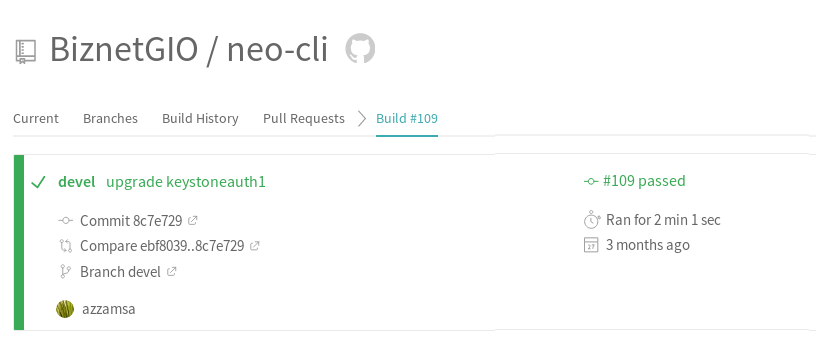
\includegraphics[width=.8\linewidth]{img/travis-head}
  \caption{\emph{Travis-ci} melaporan status pengujian}
  \label{fig:travis-head2}
\end{figure}

\subsection{Hasil Cakupan Pengujian}

Perhitugan cakupan pengujian menggunakan kakas bantu
\emph{coverage.py}. Terlihat presentase cakupan dalam Gambar
\ref{fig:test-akhir}. Status hasil pengujian juga dapat dilihat pada
gambar \ref{fig:test-akhir}.  \emph{PASSED} menandakan pengujian yang
dilakukan berhasil dan \emph{FAILED} menyatakan pengujian yang
dilakukan gagal.

\begin{figure}[H]
  \centering
  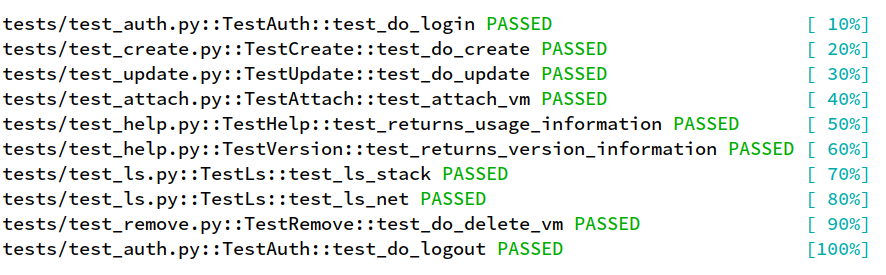
\includegraphics[width=.99\linewidth]{img/test-akhir}
  \caption{Hasil cakupan pengujian}
  \label{fig:test-akhir}
\end{figure}

%%% Local Variables:
%%% mode: latex
%%% TeX-master: "pkl"
%%% End:
